\chapter{General Setup}\label{ch:general_setup}

This chapter describes the implementation of the offloading framework in use. However, since this thesis conducts experiments both in simulation and on real robot, there are technical differences between the actual software setups. To avoid redundancies, this chapter introduces the general offloading setup in \cref{sec:general_setup:implementation} that is mutually adopted by the two setups. Furthermore, \cref{sec:general_setup:offloading_strategies} also describes the algorithms that are used to realize different offloading strategies. 
Finally, in \cref{sec:general_setup:evaluation}, this chapter discusses the evaluation paradigm in use for different evaluation metrics.

\section{Implementation}\label{sec:general_setup:implementation}

This thesis implements an offloading pipeline for a robotic object detection task. This includes an offloading module making decision whether to offloading the image from the camera sensor to the edge computer or to compute the image locally using onboard resources. An inference pipeline for object detection task is implemented using pre-trained models from YOLOv5 \cite{Jocher2022} deployed using PyTorch library \cite{Paszke2019}. Furthermore, in order to test the offloading framework in repeatable and comparable experiments, a simulation scenario is implemented in \gls{gazebo} \cite{Koenig2004} and a recording of the scenario run is created with \gls{ros}. Finally, since the output of the object detection task is not used in any downstream applications. This thesis considers and implements various evaluation paradigms to retrieve meaningful results from the data collected during the experiments. To delimit, this thesis only investigates the scenario where one \gls{amr} offloads to one edge computer. Investigations for multi-robot multi-edge scenarios are beyond the scope of this thesis. 

\subsection{Offloading Module}

\begin{figure}[htp]
    \centering
    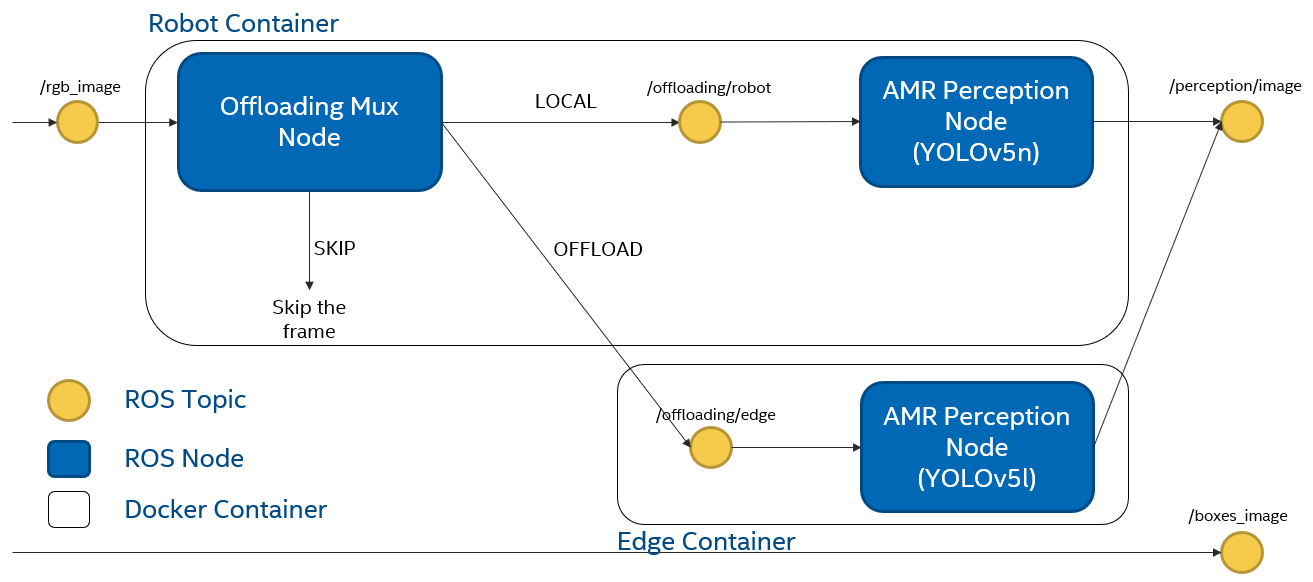
\includegraphics[width=120mm]{figures/setup/general_setup.png}
    \caption{General Setup (TODO: adapt this image)}
    \label{fig:general_setup}
\end{figure}

% TODO: this may need some adaptions to the dynamic offloading module
An offloading pipeline should have the abilities to make decision, coordinate the resources and communicate over the network. A generic offloading pipeline is illustrated in~\cref{fig:general_setup}. Each blue block represents a \gls{ros} node and each yellow circle represents a \gls{ros} topic. The arrows indicate the directions of the data flow. The dotted lines are the virtualization of the robotic system and the edge computer. The images can come from either a camera sensor or the replay of the simulation scenario. Once the \gls{amr} receives the image, the offloading module will have to decide whether to offload the image to the edge computer or pass it to the local perception node, which uses a simpler and lighter model for image inference. The offloading module makes offloading decisions by publishing the received image to pre-defined \gls{ros} topics. Once the perception nodes receive the image, they will start to do inference on the given image. Then, the processed results are published to another pre-defined \gls{ros} topic and recorded by the \gls{ros} bag. Meanwhile, the ground truth of the simulation for the object detection task is also published to a \gls{ros} topic and recorded by the \gls{ros} bag. 

In order to evaluate different offloading strategies, the offloading module possesses the ability to switch between them. Therefore, the offloading strategies act as plugins for the offloading module. Furthermore, the offloading module is responsible for loading the static hyper-parameters for the offloading strategies on start-up and also for keeping track of the run-time states of the system to allow dynamic offloading strategies. In an offloading pipeline, the system states come from various \gls{ros} nodes observing different functionalities of the system. This information is published to different \gls{ros} topics and subscribed by the offloading module. To reduce the influence of the fluctuation in the observed system states, the offloading module applies a \gls{sma} algorithm to smooth the data. 

Since the offloading pipeline is built upon the \gls{ros}, the behaviour of \gls{ros} and its underlying technical realization is crucial to the behaviour of the offloading pipeline, such as \gls{dds} and \gls{qos} settings. The exact influence of these settings on the behaviour of the offloading pipeline and the performance of the offloading will be discusses in \cref{ch:simulation} and \cref{ch:real_robot_experiment}. 

\subsection{Perception Module}

% discuss the choice of synchronous inference and asynchronous inference. Also defend not retraining the model.

% TODO: find the quote on the edge computers
In general, an offloading task can be any computationally intensive algorithms the \gls{amr} is required to run, such as perception, navigation, \gls{slam}, path planning, etc. This thesis chooses an object detection task as an example, because an object detection task can have significant performance difference between the \gls{amr}'s onboard system and the edge computer, which corresponds to the usage scenario of the edge offloading. An \gls{amr} is usually equipped with a simple onboard system with only access to \gls{cpu}, while an edge computers are usually cloudlets and data centers on premise with access to \gls{gpu}. As mentioned in \cref{ch:background}, the \glspl{amr} use primarily \glspl{dnn} to detect objects. With frameworks like PyTorch that can make use of the \gls{gpu}, the performance difference between \gls{amr}'s onboard system and the edge computer is immense. Therefore, this thesis chooses the object detection as an example for offloading tasks. 

% TODO: fill in the real value
\begin{table}[htb]%
    \centering%
    \begin{tabular}{lccccc}
        \toprule
        Model &                     YOLOv5n &   YOLOv5s &   YOLOv5m &   YOLOv5l &   YOLOv5x \\
        \midrule
        Robot inference time &      0.0 ms &    0.0 ms &    0.0 ms &    0.0 ms &    0.0 ms  \\
        Edge inference time &       0.0 ms &    0.0 ms &    0.0 ms &    0.0 ms &    0.0 ms  \\
        Model size &                0 MB &      0 MB &      0 MB &      0 MB &      0 MB    \\
        \gls{map} &                 45.7\% &  56.8\% &    64.1\% &    67.3\% &    68.9\%  \\
        \bottomrule
    \end{tabular}
    \caption{Inference times of different YOLOv5 models on \gls{amr}'s onboard system and edge computer}
    \label{tab:inference_time}%
\end{table}

% TODO: ask if it's okay to list the hardware specification
% TODO: better phrasing
In order to adapt to the performance difference between the \gls{amr}'s onboard system and the edge computer, the perception module should have two models available for object detection: a lightweight model that runs on the onboard system and a more complex model that runs on the edge computer. \gls{yolov5} provides a series of models with different complexities. To find appropriate models for the onboard system and the edge computer, this thesis investigates the inference times of different models on different machines, which can be taken from \cref{tab:inference_time}. To simulate the computation capability discrepancy between the two systems, this experiment uses a \gls{nuc} equipped with an Intel(R) Core(TM) i3-8109U \gls{cpu} and without access to \gls{gpu}. On the other hand, the edge computer is equipped with an Intel(R) Core(TM) i9-7900X \gls{cpu} and equipped with Nvidia GeForce GTX 1060 6GB \gls{gpu}. The models are deployed with \gls{pytorch} and output an array of bounding box detections. The inference time is measured between the time when the \gls{yolov5} receives the image and the time when the perception node outputs an array of bounding box detections. This includes the time for image pre-processing and the time of results post-processing. Furthermore, the image input for the offloading module has a frame rate has an average of 30 frames per second. To achieve real time, it is necessary that the inference time does not exceed 100 ms (\textbf{\textit{maybe phrase it better here}}). Longer inference time also cause the actual precision of the object detection to deteriorate, which will be discusses in \cref{sec:general_setup:evaluation}. The model sizes and the \gls{map} data are taken from the the documentation from \citeauthor*{Jocher2022} \cite{Jocher2022}. The \gls{map} data are evaluated on \gls{coco} val2017 \cite{Lin2014}. As a compromise between the inference time and the performance, this thesis chooses to deploy \gls{yolov5}n on the \gls{amr}'s onboard system and \gls{yolov5}l on the edge computer. 

To delimit, the object detection models in use are pre-trained and not re-trained with custom data from the simulation. This thesis intends to investigate different offloading strategies and generating custom data-sets and re-training the models are laborious tasks. Therefore, a re-training of the models is beyond the scope the this thesis. \citeauthor*{Jocher2022} \cite{Jocher2022} state that the all pre-trained models are trained on \gls{coco} data-sets for 300 epochs with default settings. Moreover, this thesis only considers human obstacles, which is a detection class in \gls{coco} data-sets. Therefore, the pre-trained models can provide comparability between different offloading strategies on different machines. Furthermore, re-training of the models is dependent on the quality and the size of the custom data-sets. An improper re-training can introduce additional errors or over-fitting of the models and thus determine the comparability. 

\subsection{State Monitor}

To evaluate different offloading strategies, this thesis need to get access to the system states, such as the \gls{cpu} usage, energy consumption, and network bandwidth. Various modules are implemented to measure them. 
The measurements from these modules are recorded for evaluation and also used for dynamic strategies that making decision based on run-time states of the system. However, in simulation experiments, the virtualization of the \gls{amr}'s onboard system and the edge computer is realized by the \gls{docker} containers. In contrast, different physical computers are used in the real-robot experiments. This difference in the system virtualization affects how the system states are measured. 

For simulation experiments, \gls{docker} provides the containerized system virtualization and virtual network interfaces. \citeauthor*{Ruggeri2022} \cite{Ruggeri2022} proposes that the network bandwidth in use can be measured with the network throughput. The network throughput and \gls{cpu} usage can be measured with the the statistics of the \gls{docker} containers, which is a functionality provided by \gls{docker}. Alternatively, the system states of containers can be monitored using \gls{cadvisor}. For real-robot experiments, the \gls{cpu} usage and the network throughput are measured separately on different machines using \gls{psutil} tools. In the case of Intel \glspl{cpu}, the power consumption can be measured with \gls{rapl} provided by \gls{linux} kernel Power Capping Framework. 

% TODO: not sure if this paragraph is necessary
Since it is assumed that the edge computer has abundant resources, the system states of the edge computer are not measured and are not taken into consideration during the decision-making and the evaluation process. Furthermore, even though this thesis only investigates the single-robot single-edge scenario, the available resources from the edge computers can be affected by numerous factors in real-world applications, such as the number of edge computers, the number of \glspl{amr}, and other processes running the edge computers. In addition, with more powerful hardware and easy access to power supply, the edge computer consumes more energy and computation resources for the same task than the \gls{amr}'s onboard system. Therefore, it is pointless to compare the consumption of the resources between two systems with na\"{i}vet\'{e}. In contrast, the network connection between the \gls{amr} and the edge computer is fragile and prone to disturbance. Therefore, this thesis only considers the system states of the \gls{amr}'s onboard system and the network condition between the \gls{amr} and the edge computer. 

\section{Offloading Strategies}\label{sec:general_setup:offloading_strategies}

Offloading strategies decides how the \gls{amr} offloads the computation task to the edge computer and has influence on various metrics of the system. Therefore, they are the core of the this thesis. First, this thesis investigates the static offloading strategies where the \gls{amr} offloads to the edge computer with a fixed ratio. With the results from these different offloading ratios, this thesis intends to find the limits of the system and analyze its behaviour. Then, this thesis implements an offloading strategies that uses the system states to make offloading decision dynamically with the goal to minimize the latency. 

\subsection{Static Offloading Strategy}

% This sections describes how RobotOnlyStrategy, EdgeOnlyStrategy, RatioStrategy are implemented. Include a psuedo algorithms here for RatioStrategy
\begin{algorithm}[htp]
\caption{Algorithm to offloading with a fixed ratio}\label{alg:ratio_strategy}
\begin{algorithmic}[1]
    \Function{RatioStrategy}{$r$}\Comment{where r is the offloading ratio}
        \State $c_1 \gets GetImageCounter()$\Comment{Get the counter for the total images received}
        \State $c_2 \gets GetOffloadCounter()$\Comment{Get the counter for the images offloaded}
        \State $c_1 \gets c_1 + 1$\Comment{Add one first to image counter to avoid zero division}
        \If{$c_2 / c_1 \ge r$}
            \State return false \Comment{Compute locally}
        \Else
            \State $c_2 \gets c_2 + 1$
            \State return true \Comment{Offload to edge computer}
        \EndIf
    \EndFunction
\end{algorithmic}
\end{algorithm}

This thesis first investigates the scenarios where the \gls{amr} only computes the object detection task locally on its onboard system or only offloads the task to the edge computer. Then, the thesis continues to investigate the scenarios where the \gls{amr} offloads a portion of the frames with a fixed ratio. The offloading strategies with a fixed offloading ratio can be realized with \cref{alg:ratio_strategy}. The offloading ratio should be a value ranging from 0 to 1. Any offloading ratios greater 1 will cause the offloading module only to offload to the edge computer. Accordingly, any negative offloading ratios will cause the offloading module only to compute locally.

\subsection{Dynamic Offloading Strategy}

Dynamic offloading strategies use the run-time system states to decide whether to offloading. They can adapt to the dynamic changes of the system and the network. In this thesis, we consider several run-time system states to make offloading decisions. These include the \gls{amr}'s \gls{cpu} usage, \gls{amr}'s power consumption, and the execution latency. The latency consists of two components: the network delay and the inference time. 

\section{Simulation}\label{sec:general_setup:simulation}

\subsection{Environment}

% include a bird-view shot for the simulation with warehouse, robot, and human obstacles in the view.

\subsection{Robot}

% describes how the robot is navigated, describes 

\subsection{Record and Replay}

% describes how the ROS bag is recorded and how is it replayed during the experiments and explain why this is needed. 

\section{Evaluation}\label{sec:general_setup:evaluation}

\subsection{Metrics}

% This sections lists all the evaluation metrics are used and how are they recorded and what tools are used in order to record them. 

\subsection{Synchronous Evaluation Paradigm}

\begin{figure}[htp]
    \centering
    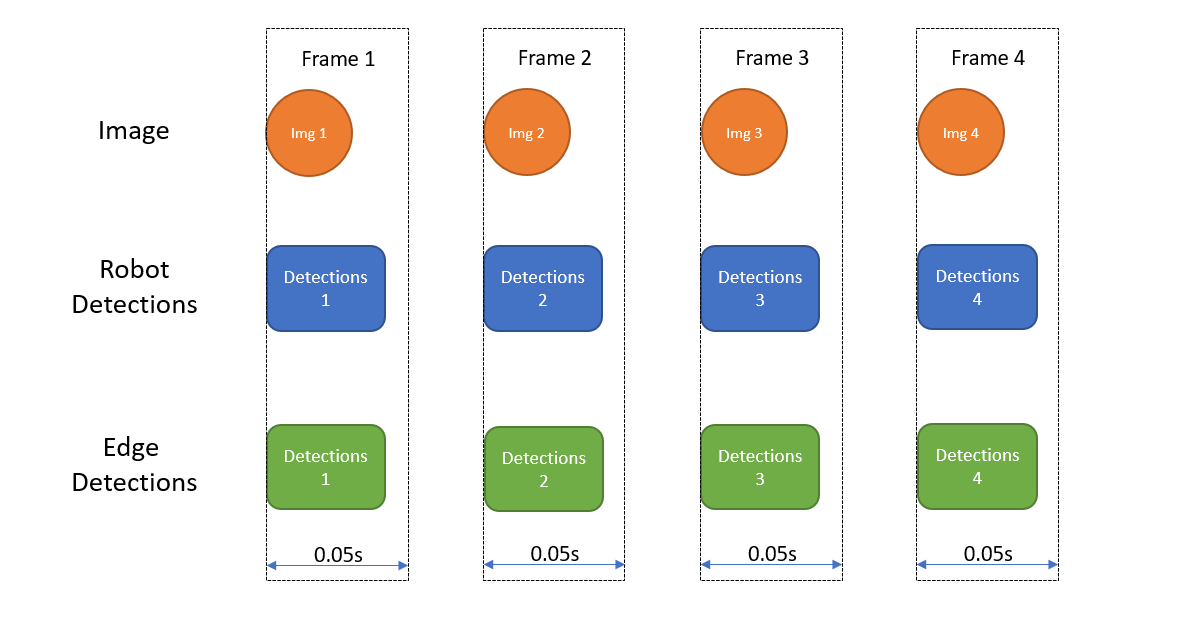
\includegraphics[width=120mm]{figures/setup/sync_eval.png}
    \caption{Synchronous evaluation paradigm}
    \label{fig:sync_eval}
\end{figure}

\subsection{Asynchronous Evaluation Paradigm}

\begin{figure}[htp]
    \centering
    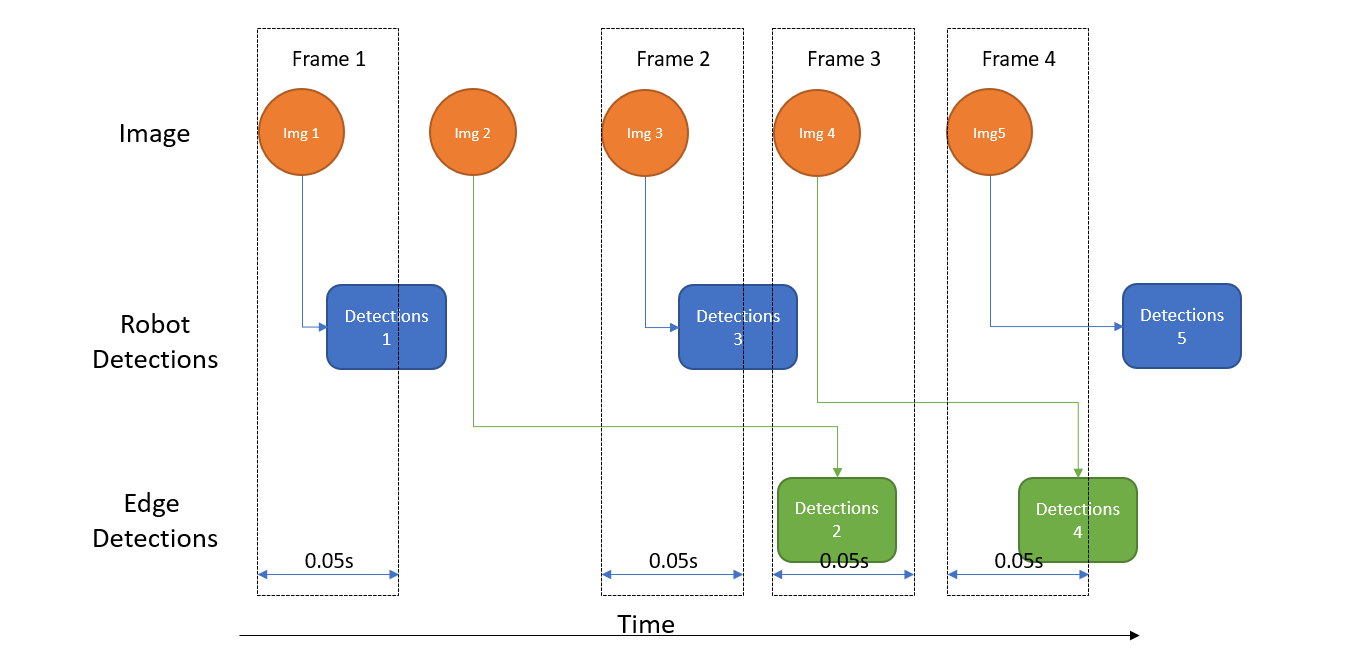
\includegraphics[width=120mm]{figures/setup/async_eval.png}
    \caption{Asynchronous evaluation paradigm}
    \label{fig:async_eval}
\end{figure}

\subsection{Discussion on Evaluation Paradigm}